\chapter {Implementácia}
Táto kapitola sa zaoberá celým procesom implementácie webovej aplikácie, od poopisu počiatočnej štruktúry projektu pri jeho inicializácii, cez zoznam použitých balíčkov s ich popisom a inicializáciou. Taktiež je venovaná pozornosť štruktúre komponentov používateľského rozhrania a implementácii aplikácie podľa prípadov použití. Koniec kapitoly sa venuje následnému nasadeniu hotovej webovej aplikácie.

\section {Počiatočná štruktúra projektu}
Implementácia webovej aplikácie započala vytvorením základnej štruktúry projektu pomocou oficiálneho nástroja pre tento účel -- \texttt{nuxi}.

Príkazom \texttt{npx nuxi init diploma-thesis} sa vytvorila zložka \texttt{diploma-thesis}, ktorej štruktúra bola nasledovná:

\begin{figure}[H]
	\dirtree{%
		.0 diploma-thesis \DTcomment{Adresár určený pre implementáciu aplikácie}.
		.1 README.md \DTcomment{Markdown súbor obsahujúci inštrukcie pre spustenie serveru}.
		.1 app.vue \DTcomment{Vue SFC súbor obsahujúci uvítaciu správu}.
		.1 nuxt.config.ts \DTcomment{Nuxt.js konfiguračný súbor}.
		.1 package.json \DTcomment{npm súbor obsahujúci popis projektu a jeho detaily s potrebnými balíčkami}.
		.1 public \DTcomment{Adresár určený pre verejne dostupný obsah}.
		.1 tsconfig.json \DTcomment{Konfigurácia TypeScriptu}.
	}
\end{figure}

\subsection {Obsah súborov projektu}
Obsahom \texttt{app.vue} súboru je Vue.js SFC komponent, ktorý reprezentuje Nuxt.js uvítaciu správu, ktorá sa zobrazí pri návšteve indexovej stránky servera.

Čo sa týka obsahu \texttt{nuxt.config.ts} súboru, ten je spočiatku prázdny. Účelom tohto súboru je konfigurácia Nuxt.js frameworku.

Pomocou súboru \texttt{tsconfig.json} je možné nakonfigurovať TypeScript pre celý projekt. Jeho počiatočným obsahom je referencia na \texttt{tsconfig.json} súbor samotného Nuxt frameworku --- čo znamená, že sa pre tento projekt aplikujú pravidlá TypeScriptu predvolené pre Nuxt.js projekt.

Jedným z najdôležitejších súborov v tejto štruktúre je \texttt{package.json}. Obsah tohto súboru definuje meno a detaily projektu spolu\newline s balíčkami, ktoré sú využité v rámci samotného projektu. Popisu použitým balíčkom sa venuje nasledujúca sekcia.

\subsection {Spustenie Nuxt.js serveru}
Pred spustením Nuxt.js serveru je potrebné doinštalovať projektové závislosti -- balíčky, príkazom \texttt{npm install}. Následne je možné spustiť Nuxt.js server príkazom \texttt{npm run dev}. Spustenie serveru týmto príkazom aktivuje tzv. \uv{file watcher}, ktorý je zodpovedný za skompilovanie aplikácie pri detekovaných zmenách v súboroch aplikácie.

\clearpage

V rámci spustenia tohto príkazu sa na konzolu vypíše adresu servera spolu s jej portom, na ktorej je možné pristúpiť k tomuto serveru. V tomto prípade sa jednalo o adresu \texttt{http://localhost:3000/}. 

Pre produkčné násadenie by mala byť Nuxt.js aplikácia najprv prejsť build procesom (pomocou príkazu \texttt{npm run build}), ktorý okrem iného minifikuje aplikačné súbory, čím zmenší prenášaný obsah aplikácie po sieti.

\section {Použité balíčky}
V rámci tejto sekcie sú uvedené všetky balíčky, ktoré sa použili pri vývoji webovej aplikácie.
Čo sa týka balíčkov, tie je možné rozdeliť na balíčky určené pre produkčné a pre vývojárske prostredie.

Zmyslom tohto delenia je definovať, aké balíčky sa majú nachádzať v produkčnej zostave aplikácie. V prípade, že je balíček pridaný do sekcie vývojárskych balíčkov, nebude sa nachádzať v produkčnej zostave. Týmto krokom sa sleduje zníženie veľkosti a zrýchlenie produkčnej zostavy projektu.

\subsection {Balíčky pre produkčné prostredie}
\texttt{cornerstone-core} -- Balíček poskytujúci Cornerstone Core knižnicu, ktorá je zodpovedná za zobrazenie DICOM snímiek v správnom formáte a jednoduchú manipuláciu s týmito snímkami.

\texttt{@tarotoma/cornerstone-tools} -- Fork \texttt{cornerstone-tools} balíčku, ktorý obsahuje rôzne nástroje určené pre prácu s DICOM snímkami. V tomto forku bol pridaný Grid nástroj implementovaný v rámci tejto diplomovej práce. Samotné knižnica taktiež upravuje prehrávanie animácií a pridáva vlastné TypeScript definície pre metódy používané vo webovej aplikácii, čo umožňuje lepšie našeptávanie IDE pri práci s týmto balíčkom.

\texttt{cornerstone-math} -- Tento balíček umožňuje použiť Cornerstone Math knižnicu v projekte. Tá slúži pre rôzne výpočty v oblasti vektorovej matematiky. V tomto prípade je táto knižnica potrebná len ako závislosť balíčka \texttt{@tarotoma/cornerstone-tools}.

\texttt{hammerjs} -- Účelom knižnice Hammer.js je pridanie podpory multi-dotykových gést pri práci s webovou apllikáciou. Táto funkcionalita nebola vo webovej aplikácii využitá, avšak je nutnou závislosťou balíčka \texttt{@tarotoma/cornerstone-tools}.

\texttt{dicom-parser} -- Dicom Parser je knižnica určená pre parsovanie DICOM súborov do štruktúrovaných objektov, s ktorými je možné ďalej pracovať.

\texttt{@cornerstonejs/dicom-image-loader} -- Cornerstone DICOM Image Loader a.k.a CDIL knižnica je určená pre importovanie DICOM súborov do webovej aplikácie. Táto knižnica umožňuje využiť Web Workers technológiu pre parsovanie DICOM súborov pomocou Dicom Parser knižnice.

\texttt{pinia} -- Pinia.js je knižnica určená pre tzv. state management aplikácie.\newline Umožňuje ukladať stav aplikácie tak, aby bol dostupný v rámci všetkých Vue.js komponentov. Bez použitia tejto knižnice by zdieľanie stavových premenných Vue.js komponentov s inými komponentami bolo komplikovanejšie a implementačne náročnejšie.

Stav aplikácie je možné rozdeliť do rôznych samostatných častí pomocou modulárnych \uv{Stores}. Tie môžu byť importované nezávisle na sebe. Knižnica je taktiež plne implementovaná pomocou TypeScriptu a ponúka podporu\newline pre konzolu prehliadača na inšpekciu aktuálneho stavu aplikácie.

\texttt{@pinia/nuxt} -- Tento balíček pridáva podporu pre integráciu Pinie do Nuxt.js aplikácie.

\texttt{vuestic-ui} -- V rámci tohto projektu sa využíva Vuestic UI kit, čo je knižnica obsahujúca rôzne UI komponenty, ktoré môžu byť importované samotnou aplikáciou. Tento UI kit bol vybraný zo subjektívneho dôvodu, nakoľko ponúka komponenty s dizajnom vhodným pre ich aplikovanie do aplikácie určenej na medicínske účely.

\texttt{@vuestic/nuxt} -- Ako už názov napovedá, tento balíček pridáva integráciu Vuestic UI kitu do Nuxt.js aplikácie tak, aby nebola potrebná jeho ďalšia konfigurácia.

\texttt{@fortawesome/free-solid-svg-icons} -- Uvedený balíček obsahuje FontAwesome\footnote{https://fontawesome.com} ikony, z ktorých sú niektoré použité v aplikácii v hornom paneli aplikácie.

\clearpage

\texttt{@fortawesome/vue-fontawesome} -- Úlohou tohto balíčka je transformovať importované FontAwesome ikony do znovupoužiteľneho komponentu, ktorý je následne možné použiť v aplikácii a pomocou neho vyrenderovať požadované ikony.

\texttt{arraybuffer-encoding} -- Tento balíček implementuje konverziu dát\newline z \texttt{ArrayBuffer} do \texttt{base64} a naspäť. Jeho využitie je popísané neskôr v rámci kompresie odosielaných dát na server.

\texttt{crypto-random-string} -- Uvedený balíček implementuje správnu podporu generovania kryptograficky silných reťazcov. Tieto reťazce sú využívané pri anonymizácií DICOM dát pred ich odoslaním na server tak, aby nebolo možné priradiť odoslanú snímku konkrétnemu pacientovi.

\subsection {Balíčky pre vývojárske prostredie}
\texttt{nuxt} -- Inštalácia tohto balíčka je nutná pre vytvorenie a vývoj v rámci Nuxt.js projektu.

\texttt{eslint} -- ESLint je open-source JavaScript nástroj, ktorý kontroluje kód a reportuje prípadné nezrovnalosti v ňom. Medzi tieto nezrovnalosti partrí nekonzistentné odsadenie kódu, či používanie jazykových konštruktov, ktoré nedodržiavajú určité jednotné pravidlá. Tieto pravidlá je možné konfigurovať,\newline ale aj importovať z iných projektov. Konfigurácia pravidiel, parsera a iných konfiguračných možností je možné pomocou \texttt{.eslintrc.cjs} súboru umiestneného v projekte.

\texttt{@typescript-eslint/parser} -- Nakoľko ESLint nepodporuje kontrolu TypeScript kódu, keďže používa Espree parser podporujúci len JavaScript, je nutné použiť tento balíček pre pridanie podpory kontroly Typescript kódu. 

\texttt{@typescript-eslint/eslint-plugin} -- Tento balíček pridáva do ESLintu pravidlá pre TypeScript kód. Použitie tohto balíčka je odporúčané pri použití predchádzajúceho balíčka.

\clearpage

\texttt{sass} -- Sass je CSS preprocesor implementovaný v JavaScripte, ktorý umožňuje vytvárať modulárnejší CSS kód, ktorý je určený pre jednoduchšie opätovné použitie. Okrem iného umožňuje používať CSS premenné, implementuje dedičnosť či vnáranie CSS pravidiel.

\texttt{sass-loader} -- Úlohou tohto balíčka je transpilovať Sass CSS kód do čistého CSS kódu, ktorý je podporovaný CSS prehliadačmi. Pri budovaní projektu je nutné akýkoľvek CSS kód vytvorený pomocou Sass transpilovať do CSS, nakoľko Sass nie je podporovaný webovými prehliadačmi.

\texttt{@types/\{cornerstone-core, hammerjs, node\}} -- Tieto tri balíčky pridávajú TypeScript definície typov \texttt{cornerstone-core}, \texttt{hammerjs} a \texttt{node} knižníc. Pridaním týchto balíčkov umožňuje používať typehinty pri práci s týmito balíčkami.

\texttt{vue-tsc} -- Tento balíček je wrapper nástroja \texttt{tsc}, pomocou ktorého je možné transpilovať TypeScript kód do JavaScriptu. Nakoľko sa v projekte využívajú Vue SFC komponenty a samotný \texttt{tsc} balíček nepodporuje kontrolu TypeScriptu v týchto komponentách, je potrebné použiť balíček \texttt{vue-tsc} miesto \texttt{tsc} pre pridanie tejto podpory. 

\section {Inicializácia vybraných knižníc}
Biznis logika spojená s akýmkoľvek Cornerstone balíčkom a ich závislosťami bude zahrnutá v rámci súboru \texttt{functions/Cornerstone.ts}. V ňom budú tieto balíčky importované a inicializované. Medzi knižnice, ktoré je nutné pred ich použitím inicializovať, patria Cornerstone Tools a Cornerstone DICOM Image Loader (CDIL). Ich inicializácia spočíva v nalinkovaní externých knižníc, ktoré dané dve knižnice využívajú v rámci ich implementácie. Bez tohto nalinkovania by niektoré metódy oboch knižníc nemuseli korektne fungovať a mohli by vyhadzovať výnimky.

Inicializácia Cornerstone Tools knižnice zahŕňa volanie metódy \texttt{init} s objektom možností, ktorú túto knižnicu pripraví pre jej použitie. Inicializácia CDIL knižnice prebieha podobne, avšak miesto  \texttt{init} používa \texttt{configure} metódiu s objektom definujúcim jej konfiguráciu.

\begin{minipage}[]{\linewidth}
\begin{minted}{typescript}
// Cornerstone.ts
import cornerstone from 'cornerstone-core';
import cornerstoneMath from 'cornerstone-math';
import cornerstoneTools from 'cornerstone-tools';
import cornerstoneDICOMImageLoader from '@cornerstonejs/dicom-image-loader';
import dicomParser from 'dicom-parser';
import Hammer from 'hammerjs';

/**
 * Initialize cornerstone libraries
 */
export const initLibraries = (): void => {
  // Setup all required cornerstone-tools dependencies
  cornerstoneTools.external.cornerstone = cornerstone;
  cornerstoneTools.external.cornerstoneMath = cornerstoneMath;
  cornerstoneTools.external.Hammer = Hammer;
  cornerstoneTools.init({
    mouseEnabled: true,
    showSVGCursors: false,
  });

  // Setup all required cornerstone-wado-image-loader dependencies
  cornerstoneDICOMImageLoader.external.cornerstone = cornerstone;
  cornerstoneDICOMImageLoader.external.dicomParser = dicomParser;
  cornerstoneDICOMImageLoader.configure({
    useWebWorkers: true,
    decodeConfig: {
      convertFloatPixelDataToInt: false,
    },
  });

  const config = {
    maxWebWorkers: navigator.hardwareConcurrency || 1,
    startWebWorkersOnDemand: false,
    taskConfiguration: {
      decodeTask: {
        initializeCodecsOnStartup: true,
        strict: false,
      },
    },
  };
  cornerstoneDICOMImageLoader.webWorkerManager.initialize(config);
}
\end{minted}
\end{minipage}

\section {Štruktúra komponentov používateľského rozhrania}
Po inicializácii projektu, inštalácii knižníc a ich inicializácii je nutné zamyslieť sa nad štruktúrou samotných Vue komponentov, ktoré budú definovať používateľské rozhranie webovej aplikácie.

Keďže z návrhu používateľského prostredia vyplýva, že rozhranie bude rozdelené na 4 hlavné časti, ponúka sa možnosť rozdeliť potrebné komponenty taktiež do 4 zložiek.

Tými budú \texttt{top-panel}, \texttt{left-panel}, \texttt{main-window} a \texttt{right-panel}. Komponenty použité v rámci jednej časti používateľského rozhrania budú spadať do danej zložky. Akýkoľvek komponent použitý vo viacerých častiach by mal byť umiestnený v zložke \texttt{general}.
Pre každú časť tohto rozhrania by mal byť taktiež vytvorený jeden hlavný komponent reprezentujúci danú časť aplikácie.

Jedná sa o nasledujúce komponenty: \texttt{TheTopPanel.vue}, \texttt{TheLeftPanel.vue}, \texttt{TheMainWindow.vue} a \texttt{TheRightPanel.vue}.

Tie budú importované v jednom entry-point komponente, ktorý bude definovať hlavnú (a jedinú) stránku aplikácie. Tento komponent bude niesť názov \texttt{index.vue} a bude umiestnený v priečinku \texttt{pages}, aby Nuxt.js spároval zobrazenie tohto komponentu pri návšteve index stránky. V tomto komponente bude taktiež importovaná metóda \texttt{initLibraries} uvedená v predchádzajúcej časti kódu. Tá bude exekuovaná v rámci metódy \texttt{onMounted}, ktorá zaručuje exekúciu kódu po tom, čo je používateľské rozhranie súčasťou Document Object Modelu (DOM) webovej aplikácie.

\clearpage

Výsledná štruktúra pre definovanie častí UI a ich komponentov je nasledujúca:
\begin{figure}[H]
	\dirtree{%
                 .0 diploma-thesis \DTcomment{Adresár určený pre implementáciu aplikácie}.
                 .1 components \DTcomment{Adresár určený pre komponenty}.
		.2 top-panel \DTcomment{Adresár pre komponenty použité v hornom paneli}.
		.2 left-panel \DTcomment{Adresár pre komponenty použité v ľavom paneli}.
		.2 main-window \DTcomment{Adresár pre komponenty použité v centrálnej časti aplikácie}.
		.2 right-panel \DTcomment{Adresár pre komponenty použité v pravom paneli}.
		.2 general \DTcomment{Adresár pre komponenty použité vo viacerých častiach aplikácie}.
		.2 TheTopPanel.vue \DTcomment{Vue SFC komponent reprezentujúci horný panel}.
		.2 TheLeftPanel.vue \DTcomment{Vue SFC komponent reprezentujúci ľavý panel}.
		.2 TheMainWindow.vue \DTcomment{Vue SFC komponent reprezentujúci centrálnu časť aplikácie}.
		.2 TheRightPanel.vue \DTcomment{Vue SFC komponent reprezentujúci pravý panel}.
		.1 pages \DTcomment {Adresár obsahujúci stránky aplikácie}.
		.2 index.vue \DTcomment {Vue SFC komponent reprezentujúci index stránku aplikácie}.
	}
\end{figure}

\section{Implementácia prípadov použitia}
Prípady použitia budú implementované podľa ich poradia, v akom boli uvedené.

\subsection {UC1 -- Zobrazenie snímiek v aplikácii}
V rámci tohto prípadu použitia je nutné implementovať import snímiek a ich zobrazenie vo webovej aplikácii.

Pred importom snímiek je potrebné označiť vybraný HTML element za element zobrazujúci importované snímky z magnetickej rezonancie. Toto označenie spočíva v zavolaní metódy \texttt{cornerstone.enable(element: HTMLElement)} Cornerstone Core knižnice.

\clearpage

Samotný import DICOM snímiek sa dá realizovať pomocou tlačidla, ktoré bude naviazané na File API, ktoré je poskytované prehliadačmi a umožňuje načítať rôzne súbory do pamäti prehliadača.

Parsovanie importovaných DICOM snímiek je možné dosiahnuť pomocou CDIL knižnice. Následne sa použije Cornerstone Core knižnica pre uloženie týchto snímiek do internej cache. To zaručí, že sa pri neskoršom zobrazovaní snímiek nemusia tieto snímky znovu načítavať, čo zvyšuje používateľský komfort pri používaní aplikácie.

Následne je možné použiť statickú metódu \texttt{displayImage} Cornerstone Core knižnice pre zobrazenie MR snímky. Tá bude vykreslená vo zvolenom označenom HTML elemente.

Bližší pohľad na algoritmus zodpovedný za import snímiek, ich parsovanie až po výsledné zobrazenie je možné vidieť na nasledujúcom sekvenčnom diagrame.

\begin {figure}[H]
        \centering
        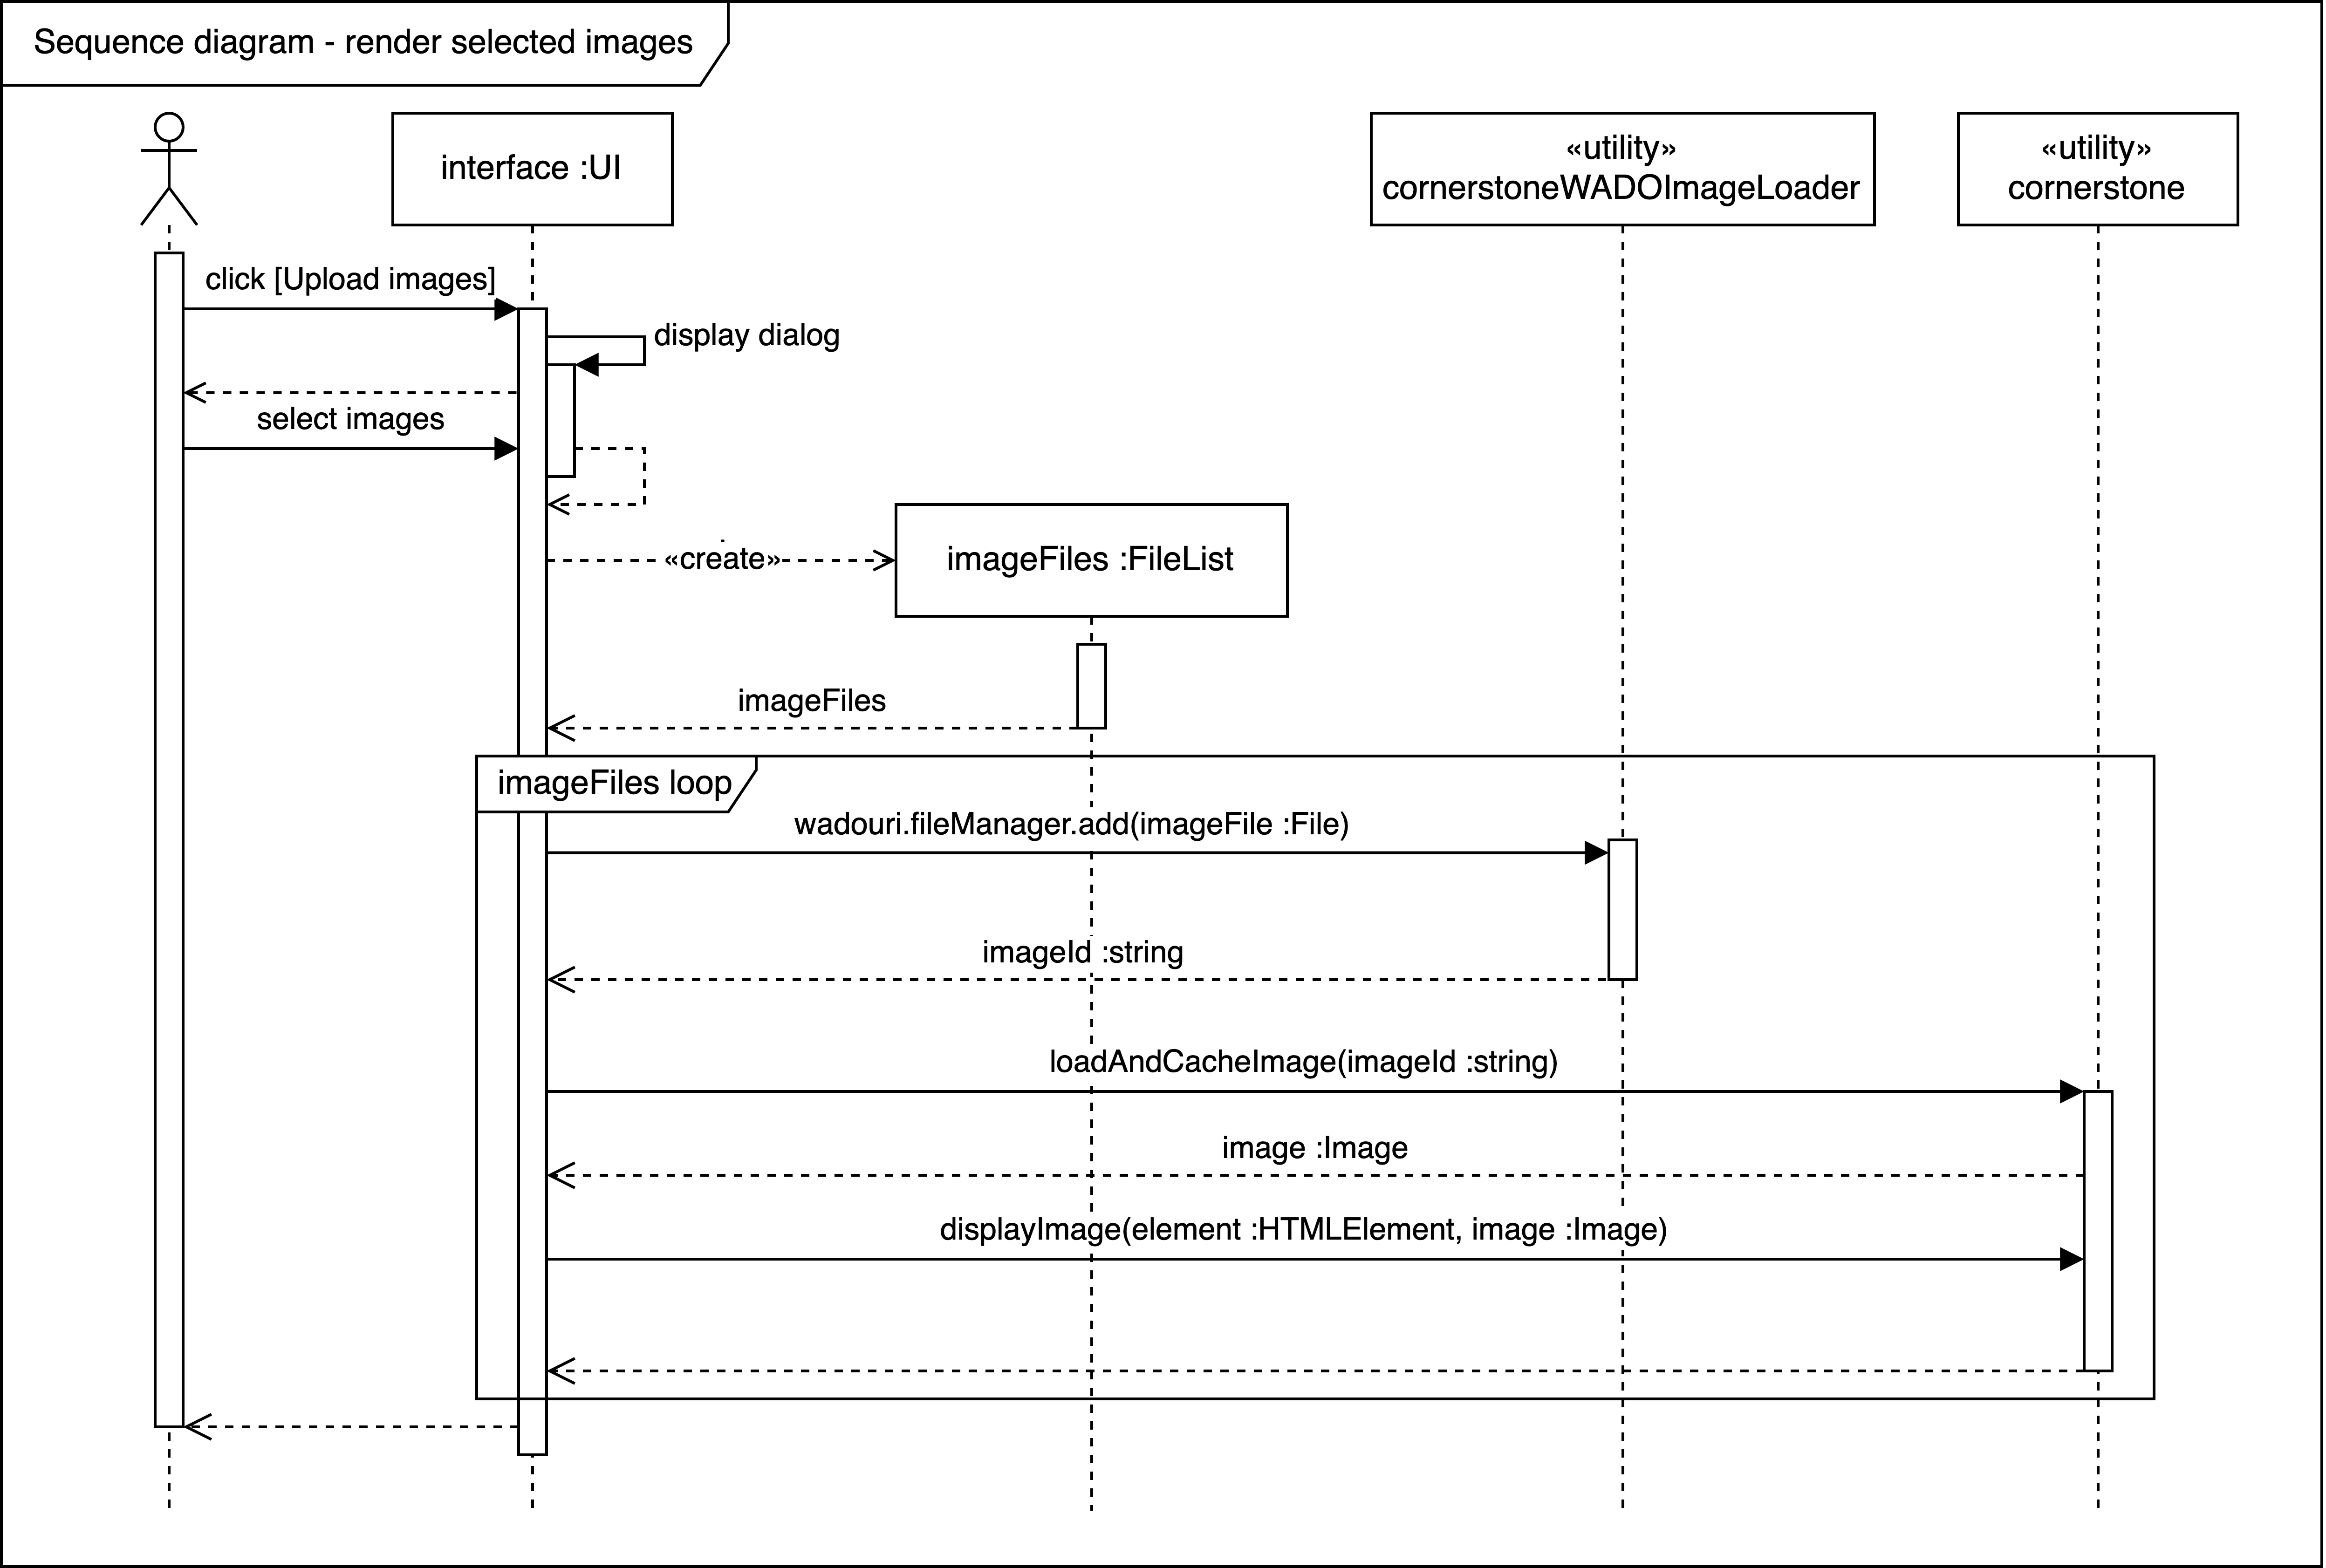
\includegraphics[height=9cm]{media/graphs/render_images.png}
        \captionsetup{justification=centering}
        \captionof{figure}{Sekvenčný diagram zobrazujúci import, parsovanie a zobrazenie DICOM snímiek}
\end {figure}

\subsection {UC2 -- Animácia snímiek}
Knižnica Cornerstone Tools ponúka nástroj \uv{PlayClip}, pomocou ktorého je možné importované snímky animovať.

Avšak po bližšej analýze tohto nástroja bolo zistené, že nie je konfigurovateľný do takej miery, ako vyžaduje alternatívny scenár tohto prípadu použitia.\newline PlayClip nástroj neprijíma indexy snímiek ako argumenty, od akej,\newline resp. po akú snímku sa animácia má prehrávať.

\subsubsection {Vytvorenie a publikácia forku Cornerstone Tools knižnice}
Táto skutočnosť viedla k potrebe vytvorenia vlastného forku Cornerstone Tools knižnice za účelom zmeny \uv{PlayClip} nástroja. Algoritmus tohto nástroja - metóda \texttt{playClip} -- bol zmenený tak, aby prijímal chýbajúce argumenty a na ich základe animoval snímky. Pomocou metódy \texttt{stopClip} je možné prebiehajúcu animáciu zastaviť.

Takto upravená knižnica bola publikovaná do npm registru pod názvom\newline \texttt{@tarotoma/cornerstone-tools}. Pre použitie upravenej knižnice v projekte je nutné zmazať existujúcu knižnicu a nahradiť ju forknutou verziou. 

Na to, aby mohol \uv{PlayClip} nástroj korektne fungovať, je potrebné ho pridať spolu s nástrojom \texttt{stack} do tzv. \uv{Stack stratégie manažovania stavu nástrojov}. K stavu nástrojov spravovaných touto stratégiou je možné pristupovať\newline z akejkoľvek snímky. Predvolene je stav nástrojov oddelený pre každú snímku, nakoľko je pri väčšine nástrojov žiaduce mať zobrazené informácie viažuce sa k danej snímke.

Okrem úpravy \uv{PlayClip} nástroja boli taktiež vytvorené TypeScript definície typov pre metódy používané webovou aplikáciou.

\clearpage

\subsection {UC3 -- Vytvorenie mriežky}
Vykreslenie mriežky nad zobrazenou snímkou patrí medzi hlavné funkčné požiadavky kladené na túto aplikáciu. Nakoľko Cornerstone Tools knižnica neposkytuje taký nástroj, bude nutné ho vytvoriť. Keďže je v projekte už použitý fork Cornerstone Tools knižnice, je priamočiarejšie implementovať tento nástroj rovno v rámci tohto forku.

Pred začatím implementácie nástroja mriežky je dôležité zoznámiť sa s anatómiou Cornerstone Tools nástrojov a jej API dokumentáciou.

\subsubsection {Popis vybraných tried nástrojov a ich metód}
Cornerstone Tools knižnica ponúka pre implementáciu anotačných nástrojov triedu \texttt{BaseAnnotationTool}, ktorá rozširuje základnú triedu nástrojov -- \texttt{BaseTool}. Nástroje implementujúce triedu \texttt{BaseAnnotationTool} umožňujú vytvárať anotácie snímiek a náležite ich upravovať \cite{base_tool_description} (vlastný preklad).

\subsubsection* {\texttt{BaseTool} trieda}
Táto trieda je zodpovedná za inicializáciu konfigurácie nástroja, dynamické aplikovanie dodatočnej funkcionality a virtuálne funkcie pre interakciu s nástrojom pomocou myši alebo dotyku \cite{base_tool_description} (vlastný preklad).

Poskytované virtuálne funkcie sú nasledovné:
\begin {itemize}
\item {\texttt{preMouseDownCallback},}
\item {\texttt{postMouseDownCallback},}
\item {\texttt{preTouchStartCallback} a}
\item {\texttt{postTouchStartCallback} \cite{base_tool_description} (vlastný preklad).}
\end {itemize}

\texttt{preMouseDownCallback} je funkcia, ktorá je spustená pred tým, ako sa začne spracovávať \texttt{mousedown}\footnote{https://developer.mozilla.org/en-US/docs/Web/API/Element/mousedown\textunderscore event} event emitovaný prehliadačom zo zvoleného elementu zobrazujúcom snímku. Predvolene táto callback funkcia nerobí nič \cite{base_tool_description} (vlastný preklad).

\texttt{postMouseDownCallback} je funkcia, ktorá je spustená po spracovaní \texttt{mousedown} eventu taktiež emitovaného zo zvoleného elementu zobrazujúcom snímku.\newline Predvolene taktiež nič nerobí \cite{base_tool_description} (vlastný preklad).

Posledné dve funkcie -- \texttt{preTouchStartCallback} a \texttt{postTouchStartCallback} sú funkcie, ktoré sú funkcionalitou podobné funkciám \texttt{preMouseDownCallback} a \texttt{postMouseDownCallback}. Rozdiel medzi nimi je ten, že zatiaľ čo prvé dve reagujú na stlačenie tlačidla myši (\texttt{mousedown} event), posledné dve reagujú\newline na dotyk dotykovej plochy (\texttt{touchstart}\footnote{https://developer.mozilla.org/en-US/docs/Web/API/Element/touchstart\textunderscore event} event) \cite{base_tool_description} (vlastný preklad).

\subsubsection* {\texttt{BaseAnnotationTool} trieda}
Táto trieda rozširuje počet virtuálnych metód o nasledujúce 4 metódy:
\begin {itemize}
\item {\texttt{mouseMoveCallback},}
\item {\texttt{handleSelectedCallback},}
\item {\texttt{toolSelectedCallback} a}
\item {\texttt{updateCachedStats} \cite{base_tool_description} (vlastný preklad).}
\end {itemize}

\texttt{mouseMoveCallback} je funkcia, ktorá sa spustí pri detekcii \texttt{mousemove}\footnote{https://developer.mozilla.org/en-US/docs/Web/API/Element/mousemove\textunderscore event} eventu. Ten je spúšťaný prehliadačom počas každého pohybu myšou \cite{base_tool_description} (vlastný preklad).

\texttt{handleSelectedCallback} je taktiež funkcia, ktorá sa avšak spúšťa po zvolení časti vykreslenej anotácie myšou alebo dotykom \cite{base_tool_description} (vlastný preklad).

\texttt{toolSelectedCallback} je funkcia, ktorá sa spustí pri zvolení daného nástroja \cite{base_tool_description} (vlastný preklad).

\texttt{updateCachedStats} funkcia je zodpovedná za aktualizáciou štatistík daného nástroja \cite{base_tool_description} (vlastný preklad).

Nakoľko sú všetky spomenuté metódy virtuálne, nemusia byť koniec koncov daným nástrojom implementované. Avšak \texttt{BaseAnnotationTool} trieda poskytuje aj abstraktné metódy, ktoré je nutné implementovať.

Ich zoznam je nasledovný:
\begin {itemize}
\item {\texttt{createNewMeasurement},}
\item {\texttt{pointNearTool},}
\item {\texttt{distanceFromPoint} a}
\item {\texttt{renderToolData} \cite{base_tool_description} (vlastný preklad).}
\end {itemize}

\texttt{createNewMeasurement} metóda je zodpovedná za vytvorenie novej anotácie a jej uloženie do pamäte. Táto metóda sa exekuuje v rámci práve aktívneho nástroja ak žiaden nástroj neodpovedal na \texttt{mousedown} event \cite{base_tool_description} (vlastný preklad).

Metóda \texttt{pointNearTool} vráti pravdivú hodnotu, ak koordináty kliknutia myšou alebo dotyku na dotykovú plochu sa nachádzajú blízko anotácie nástroja. Ak áno, tak daná časť anotácie je poslaná ako argument \texttt{toolSelectedCallback} metódy \cite{base_tool_description} (vlastný preklad).

\texttt{distanceFromPoint} metóda vracia počet pixelov medzi zadanou súradnicou a najbližšou časťou anotácie \cite{base_tool_description} (vlastný preklad).

V rámci metódy \texttt{renderToolData} je nutné implementovať vykreslenie anotácie na snímku. Samotné vykreslenie sa dá dosiahnuť pomocou interných metód ako \texttt{drawJoinedLines} pre vykreslenie úsečiek spojených v určitých bodoch či \texttt{drawHandles} pre vykreslenie bodov, ktoré môžu byť presúvané po ploche snímky \cite{base_tool_description} (vlastný preklad).

\clearpage

\subsubsection {Dostupné módy nástrojov}
Cornerstone Tools nástroje sa môžu nachádzať v štyroch rôznych módoch,\newline z ktorého je aplikovaný v čase vždy len jeden.

Zoznam týchto módov je nasledovný:
\begin {itemize}
\item {aktívny mód,}
\item {pasívny mód,}
\item {zapnutý mód a}
\item {vypnutý mód.}
\end {itemize}

Ak je nástroj v aktívnom móde, je mu umožnené zobraziť jeho obsah a meniť svoj vnútorný stav. Nástroj v tomto stave môže tiež reagovať na interakciu používateľa s týmto nástrojom \cite{cornerstone_tools_modes} (vlastný preklad).

Narozdiel od aktívneho módu, pasívny mód umožňuje všetko čo aktívny mód s tým rozdielom, že nie je možné vytvoriť nový stav nástroja (ako napr. vytvorenie novej zvislej úsečky mriežky), ale len manipulovať s jeho existujúcim stavom \cite{cornerstone_tools_modes} (vlastný preklad).

Nástroje v zapnutom móde je možné vyrenderovať, avšak nereagujú na interakciu používateľa s takýmto nástrojom. Jedná sa vlastne o taký \uv{read-only} mód nástroja \cite{cornerstone_tools_modes} (vlastný preklad).

Vypnutý mód nástroja narozdiel od všetkých uvedených módov neumožňuje s takýmto nástrojom interagovať a ani tento nástroj vykresliť. Tento mód je taktiež predvoleným módom pre každý nástroj \cite{cornerstone_tools_modes} (vlastný preklad).

Zmena režimu je možná pomocou zavolania nasledovných metód:
\begin {itemize}
\item {\texttt{cornerstoneTools.setToolActiveForElement(element: HTMLElement, toolName: string, options: object)} -- volanie tejto metódy nastaví aktívny mód nástroja pre daný element,}
\item {\texttt{cornerstoneTools.setToolPassiveForElement(element: HTMLElement, toolName: string, options: object)} -- volanie tejto metódy nastaví pasívny mód nástroja pre daný element,}
\item {\texttt{cornerstoneTools.setToolEnabledForElement(element: HTMLElement, toolName: string, options: object)} -- volanie tejto metódy nastaví zapnutý mód nástroja pre daný element a}
\item {\texttt{cornerstoneTools.setToolDisabledForElement(element: HTMLElement, toolName: string, options: object)} -- volanie tejto metódy nastaví vypnutý mód nástroja pre daný element  \cite{cornerstone_tools_modes} (vlastný preklad).}
\end {itemize}

Cornerstone Tools umožňuje danému nástroju reagovať na zmenu jeho módu pomocou nasledovných callback funkcií, ktoré je možné definovať v rámci triedy implementovaného nástroja:
\begin {itemize}
\item {\texttt{activeCallback} -- spustí sa po nastavení aktívneho módu,}
\item {\texttt{passiveCallback} -- spustí sa po nastavení pasívneho módu,}
\item {\texttt{enabledCallback} -- spustí sa po nastavení zapnutého módu a}
\item {\texttt{disabledCallback} -- spustí sa po nastavení vypnutého módu  \cite{cornerstone_tools_modes} (vlastný preklad).}
\end {itemize}

\subsubsection {Aktivácia vybraného nástroja}
Použitie vybraného nástroja je možné až po jeho registrácii.
Nasledujúca metóda \texttt{registerTool} v rámci súbora \texttt{functions/Cornerstone.ts} implementuje  túto registráciu spolu s nastavením zapnutého módu registrovaného nástroja.

\begin{minipage}[]{\linewidth}
\begin{minted}{typescript}
export const registerTool = (toolName: cornerstoneTools.ToolName): void => {
  const store = useGlobalStore() // store retrieval
  if (!store.mainImageContainer) {
    return
  }
  const fullToolName = toolName + 'Tool' as cornerstoneTools.FullToolName
  const tool = cornerstoneTools[fullToolName]
  cornerstoneTools.addToolForElement(store.mainImageContainer, tool)
  cornerstoneTools.setToolEnabledForElement(store.mainImageContainer, toolName)
}
\end{minted}
\end{minipage}

\subsubsection {Implementácia nástroja mriežky}
Grid nástroj -- nástroj mriežky -- bol implementovaný pomocou vhodného doimplementovania abstraktných a virtuálnych funkcií \texttt{BaseTool}\newline a \texttt{BaseAnnotationTool} tried uvedených v tejto práci.

V Cornerstone Tools knižnici je tento nástroj možný nájsť pod súborom\newline \texttt{src/tools/annotation/GridTool.js}. Grid nástroj bol svojou implementáciou inšpirovaný nástrojom \texttt{FreehandRoi}, ktorý umožňuje kresliť po snímku čiary rôznych dĺžok.

Taktiež boli v rámci Grid nástroja implementované pomocné metódy ako napr. metódy pre vytváranie vertikálnych úsečiek (\texttt{generateMainPrimaryLine}) a ich mazanie (\texttt{removeLastPrimaryLine}), metódy uľahčujúce prechádzanie týchto úsečiek (\texttt{getAllMainPrimaryLines}, \texttt{getPreviousPrimaryLines},\newline \texttt{getNextMainPrimaryLine}) či metódy určené pre generovanie pomocných úsečiek a ich bodov, na ktorých sa nachádzajú \uv{refinement} body\newline (\texttt{generateSubsidiaryPrimaryLines} či \newline \texttt{generateRefinementPointsOnCurrentPrimaryLines}).

Okrem horeuvedenej funkcionality je taktiež nutné myslieť na reprezentáciu mriežky ako stavu nástroja. Tomuto problému sa venuje nasledujúca podsekcia.

\subsubsection* {Reprezentácia a manažment stavu mriežky}
Stav nástrojov je možné uložiť a získať pomocou metód\newline \texttt{addToolState(element: HTMLElement, toolName: string)}\newline a \texttt{getToolState(element: HTMLElement, toolName: string)} po ich importovaní zo súboru \texttt{stateManagement/toolState.js} nachádzajúceho sa v Cornerstone Tools knižnici.

Stav mriežky je reprezentovaný poľom obsahujúcim štruktúru vertikálnych úsečiek. Jedna takáto úsečka predstavuje tzv. measurement. V rámci measurementu sú uložené body tejto úsečky. Tie obsahujú $x$ a $y$ koordináty bodu spolu s príznakom, či je daný bod hlavným (\uv{common}) bodom alebo\newline \uv{refinement} bodom.

Postupnosť uložených bodov predstavuje vertikálnu úsečku mriežky. Horizontálne úsečky budú automaticky dopočítané pri renderovaní mriežky pomocou susedných bodov priľahlých vertikálnych úsečiek.

Pri volaní metódy \texttt{createNewMeasurement} sa teda x-krát vytvorí reprezentácia vertikálnej úsečky (measurement), ktoré budú v cykle ukladané do celkového stavu mriežky pomocou metódy \texttt{addToolState}. Reprezentácia vertikálnej úsečky mriežky (tzv. \uv{measurement}) bude vyzerať nasledovne:

\begin{minipage}[]{\linewidth}
\begin{minted}[autogobble,bgcolor=white]{typescript}
{
  x: number;
  y: number;
  isCommonPoint: boolean;
}
\end{minted}
\end{minipage}
Výstup metódy \texttt{getToolState} pre mriežku bude teda nasledujúci objekt:

\begin{minipage}[]{\linewidth}
\begin{minted}[autogobble,bgcolor=white]{typescript}
{
  data: [{
    handles: {
      points: [
        {
          x: number;
          y: number;
          isCommonPoint: boolean;
        },
        ...,
        {
          x: number;
          y: number;
          isCommonPoint: boolean;
        }
      ]
    }
  },
  ...,
  ]
}
\end{minted}
\end{minipage}

\subsection {UC4 -- Úprava parametrov mriežky}
Webová aplikácia zobrazuje nielen mriežky vytvorené používateľom, ale aj mriežky prichádzajúce zo servera. Táto situácia znemožňuje si priebežne ukladať informácie o vytvorenej mriežke, nakoľko informácie o mriežke odoslanej zo serveru nebudú dostupné.

Na základe tejto skutočnosti je nutné parametre samotnej mriežky dopočítavať na základe uloženého stavu mriežky získaného pomocou už spomínanej metódy \texttt{getToolState}.

Nasledujúca sekcia sa venuje implementačným detailom týkajúcim sa zmeny konfiguráce mriežky používateľským vstupom a následnou komunikáciou aplikácie týchto zmien používateľskému rozhraniu aplikácie.

\subsubsection {Zmena konfigurácie mriežky}
Pre zmenu konfigurácie mriežky bolo nutné v jej triede vytvoriť setter metódy, ktorých úloha je úprava štruktúry mriežky podľa vstupu používateľa.

Zoznam implementovaných setter metód je nasledujúci:
\begin {itemize}
\item {\texttt{angle(value: number)} -- nastaví uhol mriežky}
\item {\texttt{moveOneHandleOnly(value: boolean)} -- nastaví mód posunu mriežky}
\item {\texttt{noOfPrimaryLines(value: number)} -- nastaví počet vertikálnych úsečiek mriežky}
\item {\texttt{noOfSecondaryLines(value: number)} -- nastaví počet horizontálnych úsečiek mriežky}
\item {\texttt{spacing(value: number)} -- nastaví rozpätie medzi hlavnými bodmi mriežky}
\item {\texttt{showRefinementPoints(value: boolean)} -- vygeneruje/zmaže \uv{refinement} body}
\end {itemize}

\clearpage

Webová aplikácia si priebežne ukladá referenciu na instanciu nástroja mriežky pomocou metódy \texttt{cornerstoneTools.getToolForElement)}, ktorej návratová hodnota je instancia nástroja. To umožňuje exekuovať implementované setter metódy nástroja mriežky priamo z Vue.js SFC komponentov.

\subsubsection {Komunikácia medzi nástrojom mriežky a používateľským rozhraním}
Pri akejkoľvek zmene v konfigurácii mriežky ako napr. zmena pozície bodu na mriežke, pridanie/odobratie vertikálnej/horizontálnej úsečky, úpravou konfigurácie mriežky alebo pri jej celkovom zmazaní je UI webovej aplikácie notifikované o zmene stavu mriežky príslušnej k zobrazenému snímku.

Táto funkcionalita je zaistená emitovaním eventov:
\begin {itemize}
\item {\texttt{cornerstonetoolsmeasurementcompleted} a}
\item {\texttt{cornerstonetoolsmeasurementremoved}}
\end {itemize}

Event \texttt{cornerstonetoolsmeasurementcompleted} taktiež obsahuje aktuálny stav mriežky.
Tieto eventy sú emitované elementom zobrazujúcim importované snímky z magnetickej rezonancie. Emitovanie týchto eventov je implementované v rámci nástroja mriežky.

Následne stačilo v komponente obsahujúcim element zobrazujúci importované snímky (\texttt{TheMainWindow.vue}) implementovať callback funkcie na horeuvedené eventy. Tieto callback funkcie sa následne postarajú o uloženie aktuálneho stavu mriežky pre zobrazenú snímku. 

Taktiež bolo potrebné nastaviť callback funkciu pre \texttt{cornerstonenewimage} event, aby sa pri zmene zobrazenej snímky uložil aktuálny stav mriežky zobrazenej na danej snímke.

\clearpage

\subsection {UC5 -- Zadanie parametrov pre SPAMM algoritmus}
Pre splnenie scenáru tohto prípadu použitia stačilo implementovať tri políčka pre zadanie čísiel. Ich hodnoty sa priebežne ukladajú do objektu, ku ktorému sa pristupuje pri posielaní dát na server za účelom výpočtu aktualizovaných koordinátov bodov mriežok.

\subsection {UC6 -- Spustenie SPAMM algoritmu a zobrazenie jeho výsledkov}
Spustenie SPAMM algoritmu je implementované zozbieraním údajov o mriežkach a importovaných snímkoch tak, aby mohli byť tieto dáta odoslané spôsobom určeným podľa návrhu komunikácie so serverom, ktorý je možný nájsť v sekcii \ref{http_request}.

\subsubsection {Vytvorenie API endpointu}
Na to, aby klient mohol komunikovať so serverom, bolo potrebné vytvoriť API endpoint podľa jeho špecifikácie v \ref{api_endpoint}.

Pre tieto účely bol vytvorený súbor \texttt{server/api/grid.post.ts}, ktorý obsahuje implementáciu daného endpointu. Telo požiadavky je daným endpointom validované --  v prípade že nevyhovuje špecifikácii tela požiadavky, server vráti chybovú správu so správou, ktorá špecifikuje jej príčinu.

Ak telo požiadavky spĺňa dané náležitosti, je požiadavka naďalej spracovávaná. Následne je poslaná odpoveď klientovi na túto požiadavku s aktualizovanými údajmi mriežok. Webová aplikácie túto odpoveď spracuje a jej obsah vykreslí pomocou delegovania tejto funkcionality Grid nástroju.

\subsubsection {Anonymizácia dát}
Pre účely anonymizácie DICOM dát bola vytvorená trieda \texttt{DicomAnonymizer}, ktorá anonymizuje všetky nájdené tagy v rámci skupín \uv{0008} a \uv{0010}.

\clearpage

V rámci konštruktoru je predaný objekt s obsahom binárnych dát DICOM súboru. Implementovaná metóda \texttt{getAnonymizedImage} vracia požadovaný anonymizovaný DICOM súbor, ktorý je následne vhodný pre jeho zaslanie po sieti. Táto metóda je exekuovaná v rámci vytvárania tela požiadavky na horeuvedený endpoint.

\section {Nasadenie aplikácie}
Pre zrhnutie je na nasledujúcom diagrame nasadenia zobrazená výsledná štruktúra nasadenia implementovanej webovej aplikácie.

Jej frontendová časť beží u klienta -- tá zahŕňa používateľské rozhranie implementované pomocou Vue.js aplikácie a manipuláciu s obrazovými dátami pomocou frameworkov rodiny Cornerstone.

V rámci backendu aplikácie beží Nitro server s implementáciou jediného API endpointu, ktorý bol uvedený vyššie.

\begin {figure}[H]
        \centering
        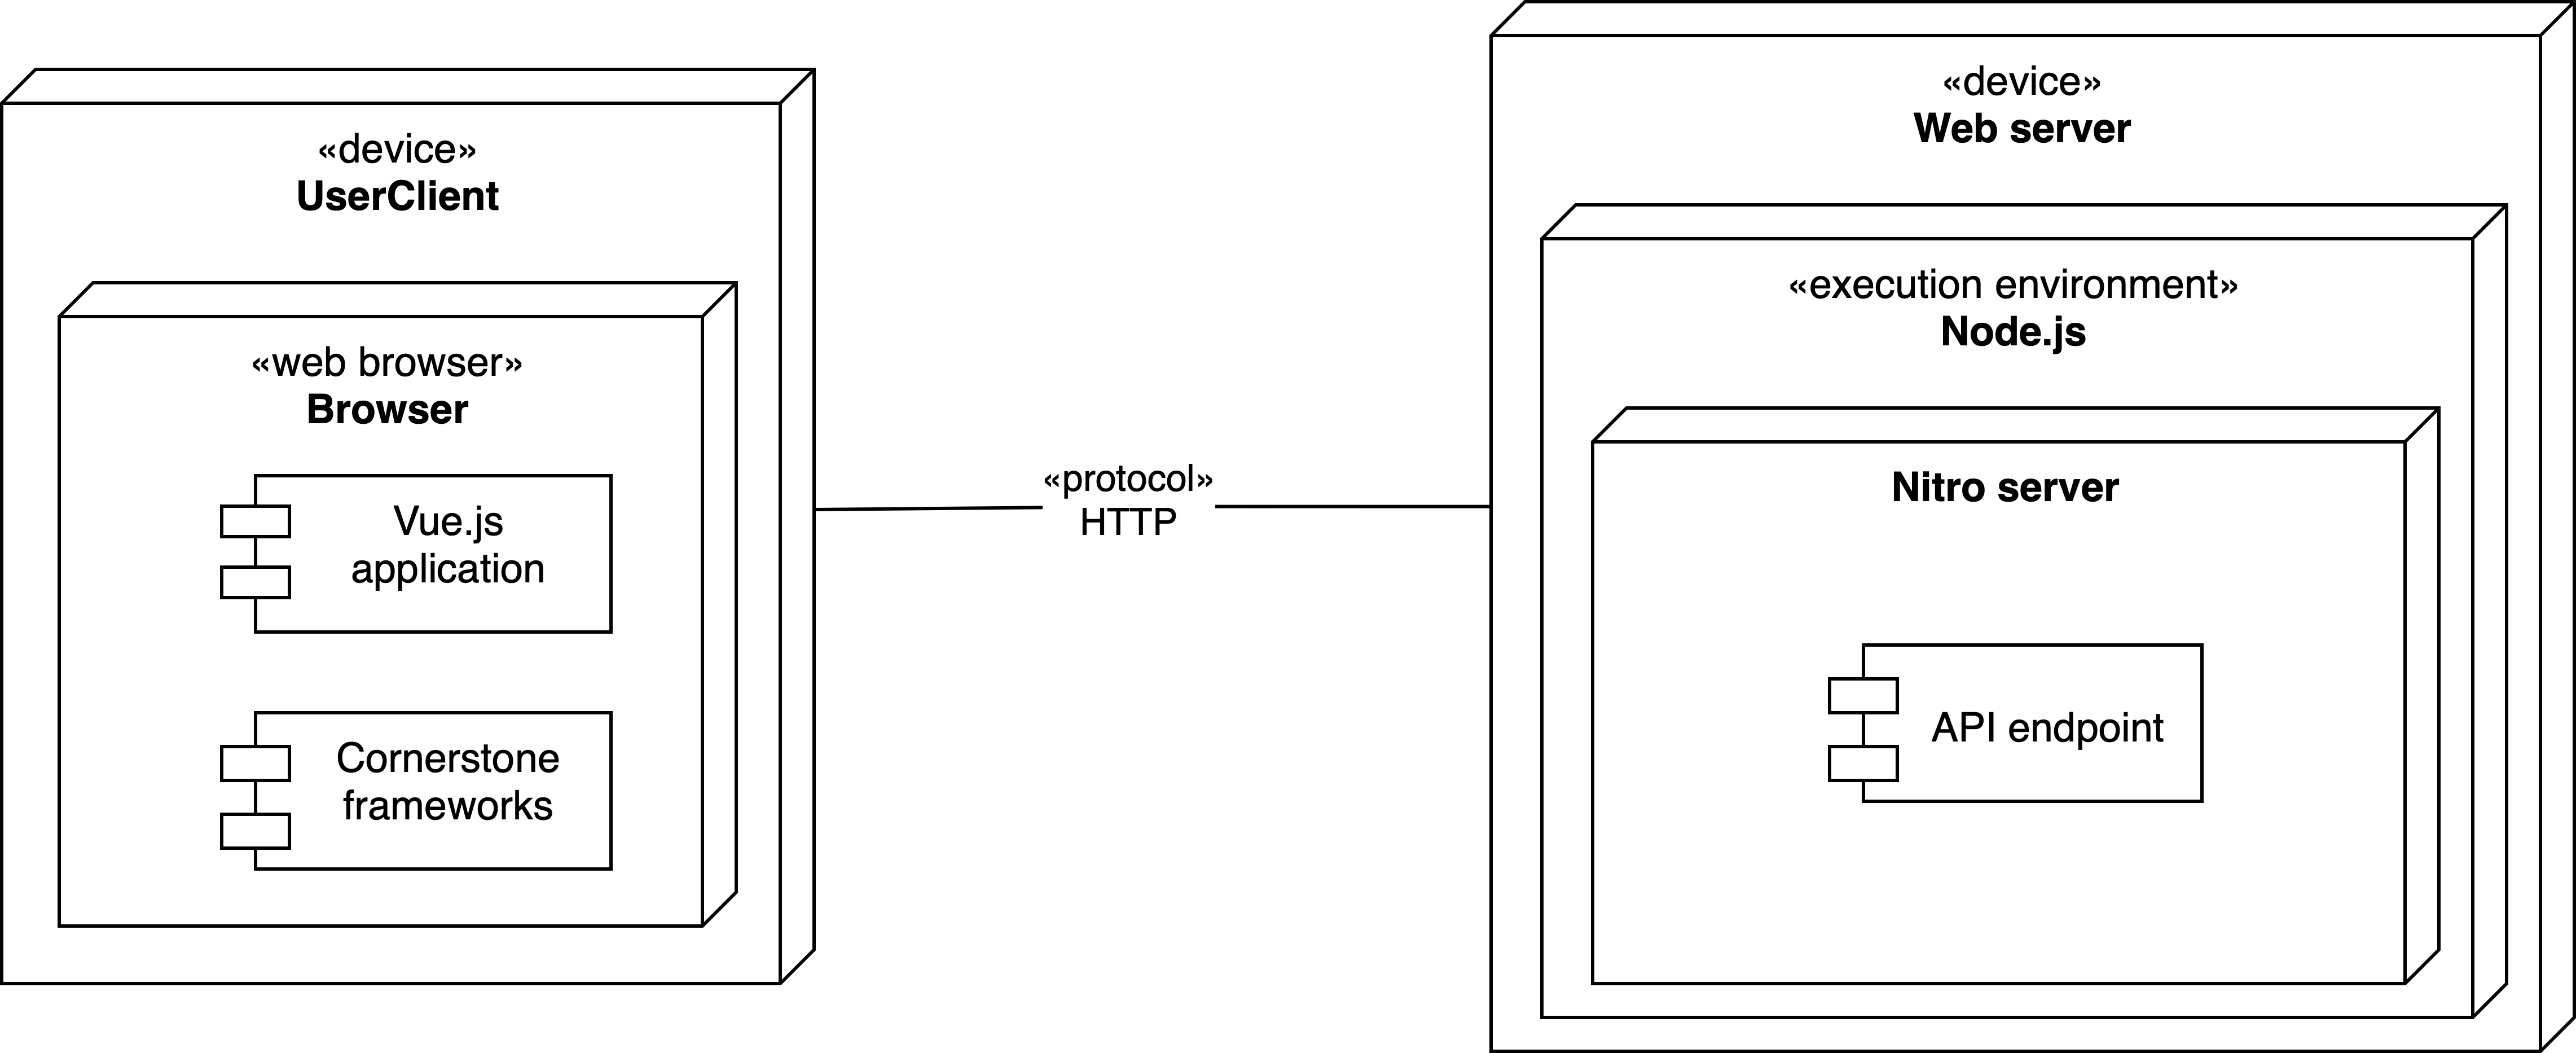
\includegraphics[height=5.4cm]{media/graphs/deployment_diagram.png}
        \captionsetup{justification=centering}
        \captionof{figure}{Diagram nasadenia zobrazujúci štruktúru webovej aplikácie}
\end {figure}

Výsledná aplikácia bola nasadená pomocou služby Vercel\footnote{https://vercel.com/}. Táto služba poskytuje aj integráciu so službou GitHub, určenou pre vytváranie \texttt{git} repozitárov.

\clearpage

Keďže bola implementovaná webová aplikácia vyvíjaná s využitím GitHubu, bola táto služba prepojená s repozitárom obsahujúcim kód tejto aplikácie. Prepojenie git repozitára a služby Vercel umožnilo automatické publikovanie aplikácie, ktoré bolo spúšťané po každej implementovanej zmene aplikácie. Tento krok umožnil mať vždy nasadenú najnovšiu verziu aplikácie online.

Potreba nasadenia aplikácie taktiež vzišla z dôvodu odtestovania implementovanej webovej aplikácie testermi a ľuďmi z IKEMu.